\documentclass{article}
\usepackage[utf8]{inputenc}
\usepackage[T1]{fontenc}
\usepackage{geometry}
\usepackage{graphicx}
\usepackage{natbib}
\usepackage{color}
\usepackage{type1ec}
\usepackage{authblk}
\usepackage{hyperref}
\usepackage{multirow}
\usepackage{booktabs}
\usepackage{setspace}

\usepackage{algorithmic}
\usepackage{algorithm}
\usepackage{subcaption}
\RequirePackage{amsmath,amssymb,amsthm,amsfonts}
\newgeometry{top=3cm,bottom=2.2cm,left=3cm,right=3cm}

\newcommand*\Bell{\ensuremath{\boldsymbol\ell}}

\title{\normalfont Genome-wide pre-miRNA discovery from few labeled examples}
\date{}
\author{C. Yones, G. Stegmayer and D. H. Milone}
\affil{\small  Research Institute for Signals, Systems and Computational Intelligence, sinc(\textit{i}), FICH-UNL, CONICET, Santa Fe, Argentina.}

\begin{document}
\setcounter{page}{73}

\maketitle

\begin{abstract}
	\noindent \textbf{Motivation:} Although many machine learning techniques have been proposed for distinguishing miRNA hairpins from other stem-loop sequences, most of the current methods use supervised learning, which requires a very good set of positive and negative examples. Those methods have important practical limitations when they have to be applied to a real prediction task. First, there is the challenge of dealing with a scarce number of positive (well-known) pre-miRNA examples. Secondly, it is very difficult to build a good set of negative examples for representing the full spectrum of non-miRNA sequences. Thirdly, in any genome, there is a huge class imbalance (1:10000) that is well-known for particularly affecting supervised classifiers.  \\
	\textbf{Results:} To enable efficient and speedy genome-wide predictions of novel miRNAs, we present miRNAss, which is a novel method based on semi-supervised learning. It  takes advantage of the information provided by the unlabeled stem-loops, thereby improving the prediction rates, even when the number of labeled examples is low and not representative of the classes. An automatic method for searching negative examples to initialize the algorithm is also proposed so as to spare the user this difficult task. MiRNAss obtained better prediction rates and shorter execution times than state-of-the-art supervised methods. It was validated with genome-wide data from three model species, with more than one million of hairpin sequences each, thereby demonstrating its applicability to a real prediction task. \\
	\textbf{Availability:} Can be downloaded from https://CRAN.R-project.org/package=miRNAss. In addition, a web-demo is available at http://fich.unl.edu.ar/sinc/web-demo/mirnass. All the datasets that were used in this study and the sets of predicted pre-miRNA are available on \\ http://sourceforge.net/projects/sourcesinc/files/mirnass \\
	\textbf{Contact:} \href{cyones@sinc.unl.edu.ar}{cyones@sinc.unl.edu.ar.} \\
	\textbf{Supplementary information:} Supplementary data are available at \textit{Bioinformatics} online.
\end{abstract}


\section{Introduction}
Over the last decade, a number of experimental and computational approaches were used to identify novel miRNAs. Experimental methods such as direct cloning are capable of detecting only abundant miRNAs \citep{kleftogiannis2013where}. Moreover, those expressed exclusively in certain stages of an organism, or in specific tissues, usually remain undetected. Most widely used approaches are hybrid computational/experimental methods, which take also advantage of the available deep sequencing data \citep{an2013mirdeep}.
The computational approaches used for pre-miRNA identification may be divided into two groups: homology search methods and machine learning methods. The first ones rely on the conservation of miRNAs between closely related species and thus cannot be used for miRNAs that are specific to one species \citep{ng2007novo}. Machine learning methods use a different approach, which involves first extracting features from the well-known pre-miRNAs, the sequences that are used as negative examples, and the unknown/unlabeled sequences to be classified.
The features that are used to represent RNA sequences were widely studied \citep{de2014discriminant, yones2015mirnafe}. After feature extraction, many types of different classifiers were applied to this problem: support vector machines, random forest, classifier ensembles, and hidden Markov models, among others \citep{kleftogiannis2013where}. The existing methods based on this supervised approach of machine learning have many drawbacks. In the first place, although the number of non-miRNA sequences that can be found in any genome is large, a recent study \citep{wei2014improved} analyzed the importance of representative negative samples in miRNA prediction and how this limits the performance of state-of-the-art methods. In most cases, the negative sets that are used to fit classification models are defined mainly with sequences taken from protein coding regions, mRNAs, or other regions where miRNAs are not expected to be found \citep{peace2015framework}. Nothing can ensure that these sequences are good representatives of all possible non-miRNA sequences, or that they are close enough to the boundaries of the true miRNA class. For example, if the prediction power of a classifier is tested on a dataset having miRNAs and ncRNAs, what is actually being measured is the capability to differentiate miRNAs from ncRNAs, but the classifier may still fail to correctly discard other non-miRNA sequences. To the best of our knowledge, no current state-of-the-art method has reported error rates considering this crucial point. Moreover, if sequences from these well-known sources of negative examples could be discarded a priori with a set of simple rules, training a model to differentiate between these two groups of sequences would be useless. To address this issue, some methods used sequences taken from random positions of a genome as negative examples \citep{wenyuan2013training,gudys2013huntmi}. However, in this case, nothing can ensure that any really novel miRNA would not be wrongly taken as a negative example. In both negative set construction strategies, the negative examples are not representative of the whole negative class; and, what is even worse, some of them might actually be false negatives.
%****************************************************************************************
\begin{figure}[tpb]
	\centering
	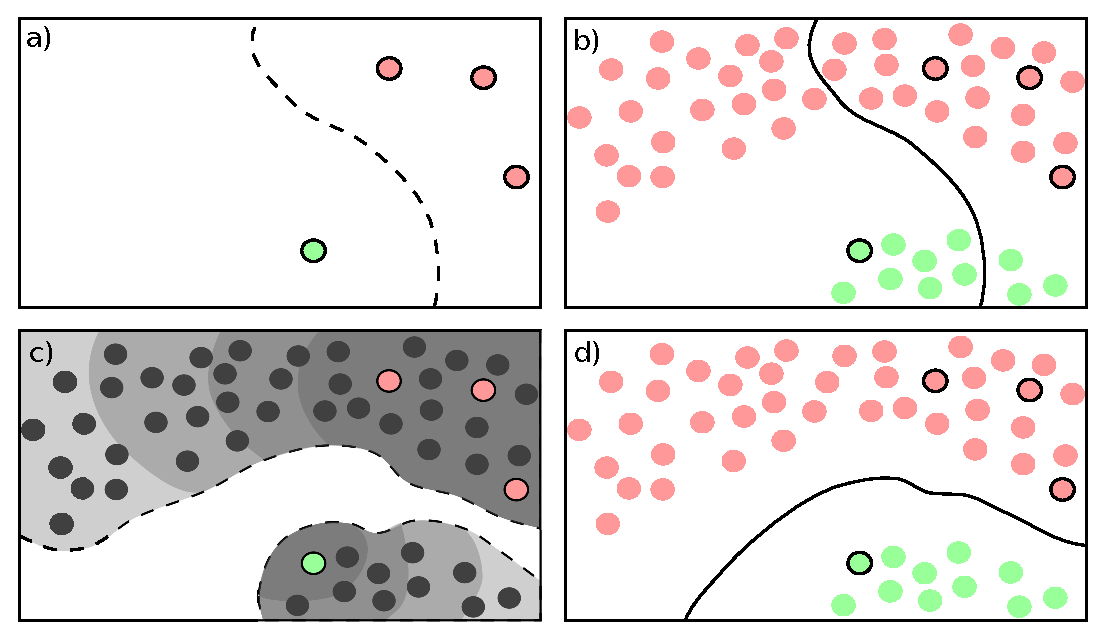
\includegraphics[width=0.6\linewidth]{supervssemi2.eps}
	\captionof{figure}{Prediction example: supervised (a-b) versus semi-supervised (c-d) approaches.}
	\label{fig:semivssuper}
\end{figure}
%****************************************************************************************

Another issue is that the existing tools are generally built using a classifier trained with a model species \citep{batuwita2009micropred} or a mixture of sequences from several species \citep{gudys2013huntmi}; however, the miRNA prediction problem is a species-dependent task \citep{de2016automatic}. Therefore, using pre-trained models cannot ensure acceptable results when predicting novel pre-miRNAs in other species that are different from the ones that were used for training. Although some tools can be re-trained, this presents some difficulties. As discussed above, negative examples are hard to define. Besides, the number of well-known positive examples is very low, since a very small proportion of true miRNAs is expected in a genome. This is an important problem in novel and non-model species, where the number of annotated pre-miRNAs might be even lower. Therefore, regardless of how negative examples are obtained or defined, and because of the natural class imbalance in any genome, thousands or even millions of unlabeled sequences are expected to be negative. This poses a high class imbalance problem, which most machine learning algorithms cannot face correctly.

In order to appropriately address these issues, we present a new method named miRNAss, which uses a semi-supervised approach to learn the latent distribution of hairpin features of the genome under analysis. This method takes advantage of unknown sequences to improve the prediction rates, even when there are just a few positive examples, and when the negative examples are unreliable or are not good representatives of its class. Furthermore, it can automatically search for negative examples if the user is unable to provide them. In addition, miRNAss automatically optimizes the threshold that defines the class boundaries and thus can separate the pre-miRNAs from other groups of sequences, in spite of the high class imbalance. Finally, we will show that the method can handle large volumes of data.

\section{Methods} \label{sec:method}
\subsection{Semi-supervised and transductive learning} \label{sec:semisupervised}
Semi-supervised learning not only uses labeled training examples but also learns from unlabeled examples to improve the classification performance. As the unlabeled examples provide extra information about the latent distribution of the data, good classification rates can be achieved even when the amount of labeled data is very low compared with unlabeled data, or when it is unrepresentative of its class \citep{chapelle2006semi}.
%****************************************************************************************
\begin{figure}[tpb]
	\centering
	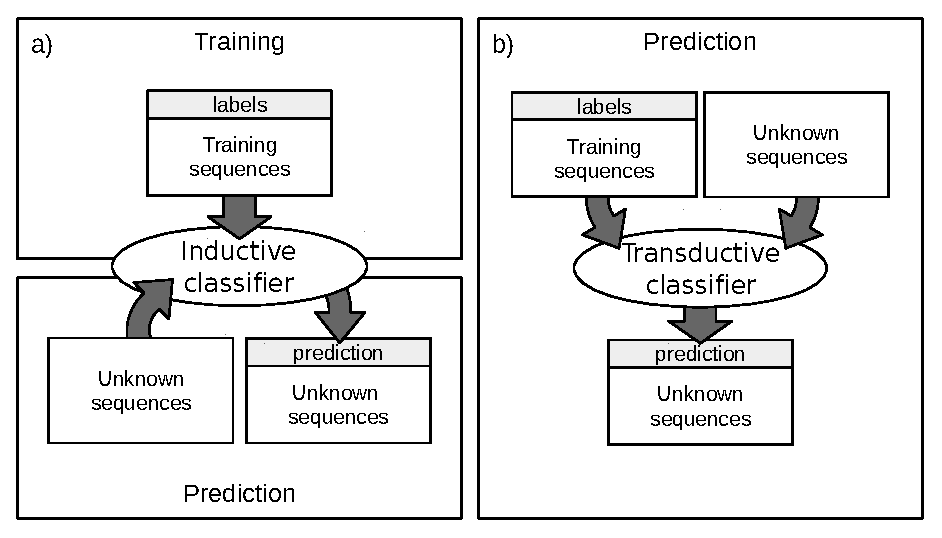
\includegraphics[width=0.6\linewidth]{paradigmas.eps}
	\caption{Inductive and transductive learning. a) Traditional inductive scheme with two separate stages; b) Transductive scheme with only one stage.}
	\label{fig:schemes}
\end{figure}
%****************************************************************************************
Fig.~\ref{fig:semivssuper} shows a very simple scenario with four labeled examples for training: three negative examples (in red) and one positive example (in green). If a classic supervised method is used here, a decision boundary like the dashed line in Fig.~\ref{fig:semivssuper}.a is obtained. This classifier fails over the unknown sequences (Fig.~\ref{fig:semivssuper}.b), because the training sequences are very few and actually unrepresentative of each class. If a semi-supervised scheme is employed instead (Fig.~\ref{fig:semivssuper}.c), it is observed that it has access to both labeled and unlabeled sequences, all together at the same time, where two real groups are hidden beneath the latent distribution of the data. Thus, the semi-supervised predictor can successfully separate the two classes (Fig.~\ref{fig:semivssuper}.d).

The concept of transductive learning is closely related to semi-supervised learning. In this setting, specific training cases are used to directly make inferences on test cases. Unlike most common inductive methods, where the algorithm has two stages (training and testing), transductive methods have only one stage, as shown in Fig.~\ref{fig:schemes}. In the inductive scheme (a), the learning algorithm uses training sequences, all labeled, to fit a model. In the second stage, the fitted model is used to make a prediction over unknown sequences. In the transductive scheme (b), both labeled and unlabeled sequences are processed together, in the same stage. As a result, a prediction over the unlabeled sequences is obtained, but no decision function, trained model, or classification rule are returned as output. While an inductive method infers a decision function that can be used to predict labels of any sequence, the transduction model directly estimates the set of labels for the unknown sequences \citep{chapelle2006semi}.
Nevertheless, a transductive classifier can be analyzed after training similarly to an inductive one. For example, in a graph based method, the adjacencies among the samples labeled in the transductive stage could be used for knowledge extraction \citep{enright2001biolayout,novak2010graph}. The semi-supervised method proposed in this work uses such transductive scheme. Therefore, training examples and unknown sequences are processed together, every time a prediction has to be made. This is not a problem in pre-miRNA prediction, because it is preferable for the model to be fed with all the sequences from the species under study (or a closely related one) in order to learn its specific characteristics \citep{de2016automatic}.
It should be noted that the validation of any transductive method is quite different from a standard (inductive) one. Since training and prediction are combined in one stage, training sequences are provided with labels, and test data are also given but \textit{without} labels. This special kind of validation is used in all semi-supervised algorithms \citep{chapelle2006semi}, where the labels of test cases are never used in any step of the prediction stage.

\subsection{The miRNAss method} \label{sec:miRNAss}
Over the last decade, one of the most active areas in semi-supervised learning has been based on graphs, where each node represents a data point, and an edge connects nodes if they are in some way similar. Then, using the labeled nodes, predicted labels are obtained for the rest of the unlabeled nodes. These methods have shown good prediction rates \citep{joachims2003transductive} and have been able to handle large volumes of data, because they can be implemented using a sparse matrix in $\mathcal{O}(n)$ memory, with $n$ number of analyzed sequences. The most computationally expensive part is the graph construction; however, this can be done by brute force in $\mathcal{O}(n^2 \log n)$, calculating the distances between all sequences and searching for the smallest $k$ for each one in$\mathcal{O}(\log n)$.
%****************************************************************************************
\begin{figure}[tpb]
	\centering
	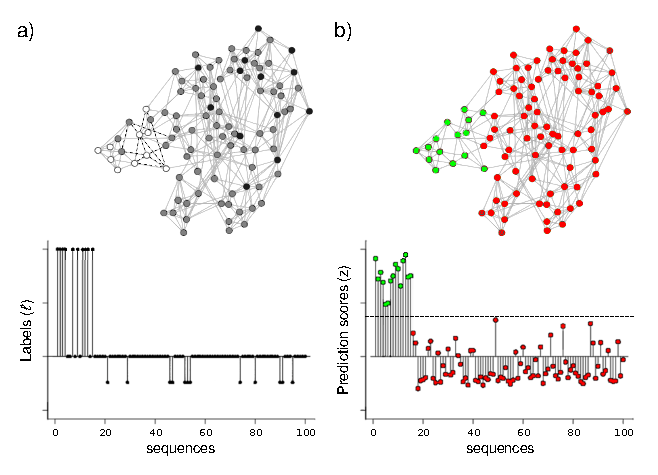
\includegraphics[width=0.6\linewidth]{workflow.eps}
	\caption{Evolution of the graph, the label vector, and the vector of prediction scores in the two steps of miRNAss: a) Graph construction and negative set initialization; b) Estimation of prediction scores and thresholding.}
	\label{fig:workflow}
\end{figure}
%****************************************************************************************
MiRNAss receives as input a set of $m$-dimensional feature vectors $\mathbf{x}_{i}$, which represent sequences, and a corresponding vector of labels $\Bell$. The $i$-th element in the vector of labels has a positive value $\gamma_{+}$ if the $i$-th sequence is a well-known pre-miRNA, a negative value $\gamma_{-}$ if it is not a pre-miRNA, and zero if it is an unknown sequence that has to be classified (predicted) by the method. The method has four steps: 1) construction of a graph where each node represents a sequence; 2) search for negative examples, if they are not provided; 3) estimation of the prediction scores for each node in the graph; and 4) estimation of an optimal threshold to finally separate the sequences into two classes. Each step is explained in detail in the following subsections.

Fig.~\ref{fig:workflow} shows an example of the evolution of the method. In this example, 15 sequences are true pre-miRNAs and the rest are non-miRNA sequences. In Fig.~\ref{fig:workflow}.a, the graph is constructed and $\Bell$ has positive values ($\gamma_{+}$), representing the well-known pre-miRNAs examples. In addition, some nodes that are topologically far from the positive examples are labeled as negative examples ($\gamma_{-}$). The nodes of the graph are colored according to the values in the $\Bell$ vector. In  Fig.~\ref{fig:workflow}.b, prediction scores are estimated for all the sequences, taking into account that: i) they have to be smooth; that is, topologically close sequences in the graph must have similar prediction scores; and ii) the scores have to be similar to the non-zero values given in the label vector $\Bell$. Finally, using the prediction scores assigned to the labeled examples, an optimal threshold is estimated in order to separate the pre-miRNAs from the other sequences. The sequences that pass the threshold are colored in green; the rest, in red.

\subsubsection{Graph construction}
To build the graph, each node represents a sequence, and an edge joins two nodes if the sequences can be considered similar. The euclidean distance between the feature vectors is used to make this measurement. If a feature does not really help to discriminate between classes, it may worsen the performance of the classifier. Therefore, it is important to pre-process the feature vectors to properly weight each feature according to its prediction power. An algorithm that has shown to improve results in classifiers that are sensitive to distance function is the RELIEF-F algorithm \citep{kononenko1994estimating, wettschereck1997review}. Furthermore, it is computationally efficient and can be used for large volumes of data.
It  works as follows: starting with a vector of weights with $m$ zeros, for each example it searches for the closest same-class example and the closest different-class example. Then, it increases the weights of features that are similar to the same-class example and different to the different-class example. Conversely, the weights of features that are different to the same-class example or similar to the different-class example are decreased. The result is called relevance vector and has high values for the most discriminative features. If the relevance of a feature is negative, it does not help to discriminate between classes; therefore can be removed. The rest of the features are scaled by their relevance score in order to give more weight to the most discriminative ones.

For graph construction, a common choice is the k-nearest neighbors (KNN) algorithm, because it is simple, fast, memory-efficient, and easily parallelizable. KNN constructs a similarity-weighted matrix
\begin{equation}
	a_{ij} =
	\begin{cases}
		\frac{\mu}{\mu + ||\mathbf{x}_{i} - \mathbf{x}_{j}||^2} & \text{if} \ \mathbf{x}_{j} \in  \mathcal{K}(\mathbf{x}_{i}) \ \text{and} \ \ell_{i} \ell_{j} \geq 0 \\
		0 & \text{in other cases,} \\
	\end{cases}
\end{equation}
\noindent where $\mathbf{x}_{i}$ is the feature vector corresponding to the $i$-th sequence, $\mathcal{K}(\mathbf{x}_{i})$ is the set of the k-nearest neighbors of $\mathbf{x}_{i}$, and $\mu$ is the mean of the distances between the connected sequences used to normalize the edge weights.


\subsubsection{Automatic search for negative examples}
If only positive examples are provided, the graph adjacency matrix  can be used to label a set of  sequences as negative. The key idea is to randomly select some unlabeled sequences among the most dissimilar from the positive examples. That way, the probability of incorrectly labeling a well-known pre-miRNA as a negative example will be low. For that purpose, a measure of the similarity of each sequence to the positive examples is calculated using the topological distance. This similarity vector, called $\mathbf{s}$, is defined $+1$ in the elements corresponding to positive examples. The unlabeled nodes are initialized to $0$. Then, an iterative method can be used to update the similarities in $\mathbf{s}$ (see Algorithm~\ref{algNS}). In each iteration and for every node, the corresponding similarity of each neighbor is multiplied by the corresponding edge weights that connect them. The maximum value from the results obtained for each neighbors is then compared with the current similarity value of the node. If it is higher, the similarity value of the node is updated. When there are no more changes in $\mathbf{s}$, $T$ sequences are sampled using $p_{i} = e^{1 - s_{i}} -1$ and labeled as negative examples.
%****************************************************************************************
\algsetup{indent=3em}
\renewcommand{\algorithmicrequire}{\textbf{Input:}}
\renewcommand{\algorithmicensure}{\textbf{Output:}}
\renewcommand{\baselinestretch}{1.5}
\begin{algorithm}[tpb]
	\caption{Automatic search for negative examples}
	\label{algNS}
	\begin{algorithmic}[1]
		\REQUIRE{adjacency matrix $A$, label vector $\Bell$ with zeros and positive values only and the number of negative examples to label $T$.}
		\ENSURE{the vector $\Bell$ with $T$ negative labels assigned.}
		\STATE{$s_{i} = \begin{cases}
				1 & \text{if} \quad \ell_{i} > 0 \\
				0 & \text{in other cases} \\
		\end{cases}$}
		\REPEAT
		\STATE{$s_{i} = \max_{\forall j \neq i}\limits \, \{s_{i}, a_{ij} s_{j} \}, \quad \forall i$}
		\UNTIL{there are no changes in $\mathbf{s}$}
		\STATE{$p_i=e^{1-s_i}-1,\quad \forall i$}
		\STATE{Sample $T$ elements of $\Bell$ using $\mathbf{p}$ as selection weights}
		\STATE{Label selected elements as negative class}
		\RETURN $\Bell$
	\end{algorithmic}
\end{algorithm}
%	%****************************************************************************************

\subsubsection{Estimation of the prediction scores}
In the third step, the prediction scores are calculated by solving an optimization problem \citep{joachims2003transductive}. As stated earlier, two points should be considered: i) the prediction scores must be topologically smooth; and ii) the predictions must be similar to the known labels. To make prediction smooth, the square of the differences between the prediction scores of adjacent sequences is minimized. A convenient representation for easily calculating these differences is the normalized Laplacian graph \citep{shi2000normalized}, defined as $L = I- D^{-1/2} A D^{-1/2}$, where $D$ is the degree matrix defined as $d_{ij} = \sum_{k=0}^n a_{ik}$ if $i=j$, and zero in other cases. The Laplacian graph has a useful property for measuring the smoothness of the solution. Suppose $\mathbf{z} \in \mathbb{R}^N$, with one prediction for each node of the graph. Then,
\begin{equation}
	\begin{split}
		\mathbf{z}^T L \mathbf{z} & = \mathbf{z}^T I \mathbf{z} - \mathbf{z}^T {D^{-1/2}}^T A D^{-1/2} \mathbf{z} = \\
					  & = \sum_{i}^{n} z_{i}^{2} -  \sum_{i}^{n}  \sum_{j}^{n} \frac{z_{i}}{\sqrt{d_{ii}}} \frac{z_{j}}{\sqrt{d_{jj}}} a_{ij} = \\
					  & = \frac{1}{2} \sum_{i}^{n} \sum_{j}^{n} a_{ij} \left(\frac{z_{i}}{ \sqrt{d_{ii}}} - \frac{z_{j}}{\sqrt{d_{jj}}} \right)^{2}.
	\end{split}
\end{equation}
\noindent This last expression shows that $\mathbf{z}^T L \mathbf{z}$ measures the squared difference between predictions $z_{i}$ and $z_{j}$, weighted by $a_{ij}$. If sequences $i$ and $j$ are similar, and thus $a_{ij}$ has a relative high value, any difference between the two predictions will have a high cost. If there is no edge connecting the two sequences, $a_{ij}=0$ and the difference between predictions is ignored. Furthermore, it should be noted that predictions are weighted by the inverse of the square root of the node degree. As a result, nodes with a small degree are considered as important as highly connected nodes.

To minimize the inconsistency between predictions and well-known labels, the squared difference between predictions and non-zero labels in $\Bell$ is also required in the objective function. Therefore, it has two terms: the first term measures the non-smoothness of the solution using the normalized Laplacian matrix (unsupervised component), and the second term is the squared difference between predictions and non-zero labels in $\Bell$ (supervised component). To take full advantage of the semi-supervised learning, there should not be strong overlap between the classes to be separated. Nevertheless, if this prerequisite is not fulfilled, the method behaves as any other supervised method in the same conditions. If there is not any clear separation, the first term of the objective function will not have any sharp minimum. Therefore, the second term of the equation (the supervised one) will lead the search. The full optimization problem is defined as
\begin{equation}
	\begin{split}
		\arg\min_{\mathbf{z}} & \qquad \mathbf{z}^TL\mathbf{z} +c(\mathbf{z}-\Bell)^TC(\mathbf{z}-\Bell) \\
		s.t. & \qquad \mathbf{z}^T\mathbf{1} = 0, \mathbf{z}^T\mathbf{z} = n,
	\end{split}
\end{equation}
\noindent where the combination of both restrictions avoids trivial solutions. In the first restriction, the sum of elements of $\mathbf{z}$ is required to be zero; that is, the prediction labels need to have both negative and positive values. The second restriction eliminates scaled versions of the solution that, for our purpose, are all equivalent.
The values $\ell_{i}$ are set to $\gamma_{+}$, $\gamma_{-}$, or zero, depending on whether the $i$-th sequence is a positive, a negative, or an unknown example, respectively. As the objective function forces the values of $\mathbf{z}$ to be close to $\gamma_{+}$ or $\gamma_{-}$, these constants have to be defined such that the optimal solution $\mathbf{z}^\star$ be able to satisfy both restrictions of the problem. If $n_{+}$ and $n_{-}$ are the true numbers of positive and negative nodes in the solution, defining $\gamma_{+} = \sqrt{n_{-} / n_{+}}$ and $\gamma_{-} = - \sqrt{n_{+} / n_{-}}$ makes $\mathbf{z}^\star$ satisfy both restrictions. This can be observed by replacing $\mathbf{z}^\star$ in the restrictions and assuming that this vector has $n_{+}$ elements equal to $\gamma_{+}$ and $n_{-}$ equal to $\gamma_{-}$. The numbers $n_{+}$ and $n_{-}$ are usually unknown, but they can be easily estimated from the training examples. If positive and negative examples are provided for training, miRNAss will estimate $n_{+}/n_{-}$ as the proportion of examples given. If there are only positive examples, $n_{+}$ is estimated as twice the number of training sequences and $n_{-} = n - n_{+}$. This estimation could be improved using domain knowledge, that is, using the expected number of well-known miRNAs for a given species; however, it is not necessary as miRNAss is not sensitive to these parameters (see Figure~S1 in Supplementary Material). Therefore, any value between the number of positive training sequences and four times this number can be used without impact in performance. By default, twice the number of positive training sequences is used as an intermediate value.
The constant $c$ in the objective function can be used to set the relative weight of the second term compared with the first one. A large value of $c$ gives a higher penalization to the misclassifications, pushing the prediction scores to values similar to the non-zero labels $\Bell$. Conversely, if a low value of $c$ is used, the misclassifications are less penalized and the first term dominates the objective function, thus producing a smoother solution. Matrix $C$ in the second term is a diagonal matrix that is zero-valued in the elements corresponding to unknown sequences. This way, the unlabeled sequences are ignored in this term. In the non-zero elements (corresponding to the labeled examples), the value assigned allows different misclassification costs per sequence. This weighting can be used, for example, to assign lower values to pre-miRNAs that have not been experimentally validated or that are unreliable negative examples. It can also be used to avoid misclassification of labeled examples. In Section S2 (of the Supplementary Material) it is proved that if $C_{ii} > (n n_{+}) / (c n_{-})$, misclassifying the $i$-th sequence will have a greater penalization than any penalization in the not supervised term. Then, it cannot be misclassified. As a default value, the non-zero elements of $C$ are set to $1$, for both positive and negative examples.

To solve this optimization problem, we first calculate the spectral decomposition of the Laplacian $L = U \Sigma U^T$. Next, we introduce a new parameter vector $\mathbf{w}$ and replace $\mathbf{z} = U \mathbf{w}$. Since the eigenvector corresponding to the lowest eigenvalue is always constant, the first constraint of the optimization problem becomes equivalent to $w_{1}=0$. If we define $V$ as the matrix with all the eigenvectors except the first one, and $H$ as the diagonal matrix with all eigenvalues except the lowest one, we get the following optimization problem
\begin{equation}
	\begin{split}
		\arg\min_{\mathbf{w}} & \quad \mathbf{w}^T H \mathbf{w} + c (V \mathbf{w} - \Bell)^T C (V \mathbf{w} - \Bell) \\
		s.t. & \quad \mathbf{w}^T \mathbf{w} = n.
	\end{split}
\end{equation}
\noindent Defining $Q = H + c V^T C V$ and $b = c V^T C \Bell$, this problem can be rewritten as
\begin{equation}
	\begin{split}
		\arg\min_{\mathbf{w}} &\quad \mathbf{w}^T Q \mathbf{w} + 2 b^T \mathbf{w} + c \Bell^T C \Bell \\
		s.t. &\quad \mathbf{w}^T \mathbf{w} = n,
	\end{split}
\end{equation}
\noindent where the last term can be dropped since it is constant. Using Lagrange multipliers, the global minimum of this function occurs in $\mathbf{w}^\star = (Q - \lambda^\star I)^{-1} \mathbf{b}$. Now, using the results of \citep{gander1989constrained}, $\lambda^\star$ can be calculated as the lowest eigenvalue of
\begin{equation}
	M = \left( \begin{array}{cc}
			Q & -I \\
	\frac{{\mathbf{b} \mathbf{b}^T}}{{n}} & Q \end{array} \right).
\end{equation}
%*****************************************************************************************
From this solution, the predicted labels are calculated as $\mathbf{z}^\star = V \mathbf{w}^\star$.

\subsubsection{Thresholding the prediction scores}
Given the high imbalances that are present in genome-wide data, increasing the misclassification cost of the positive class is mandatory. While matrix $C$ can be used to assign different misclassification costs in the optimization process, estimating the threshold to be applied in $\mathbf{z}$ may be a more flexible and efficient method for maximizing a given performance measure. Since the prediction scores are expected to rank sequences properly, thresholding the results of the prediction scores is equivalent to classifying with weighted costs \citep{mease2007boosted}. In addition, depending on the user's needs, different performance measures may be selected for optimization after the prediction scores are calculated.

A common assessment metric that is used in class imbalanced problems is the geometric mean ($\bar{G}$) of the sensitivity and the specificity $\bar{G} = \sqrt{S^{+} S^{-}}$ \citep{batuwita2009micropred,gudys2013huntmi}, where $S^{+}$ is the proportion of positive sequences correctly classified as positive (sensitivity), and $S^{-}$ is the proportion of negative sequences correctly predicted as negative (specificity). This measure has the advantage of giving the same importance to both negative and positive classes, regardless of the number of elements in each class, and it will be used for a fair comparison with previous method. A better metric is the \mbox{F-measure} $F_{1} = 2 \, P \, S^{+}/(P + S^{+})$, where $P$ is the precision, that is, the proportion of true positives within the sequences classified as positive. When $F_{1}$ is used for threshold optimization, it  gives a better $P$ at the cost of a lower $S^{+}$. Given the large class imbalances in the pre-miRNA prediction problem, it is important to take into account the number of false positives. Therefore, $F_{1}$ is a better measure for this problem. To find a threshold, the prediction scores obtained for labeled examples may be used to estimate the target measure of performance. It should be pointed out that this is only an estimation, since the unlabeled sequences cannot be used. For this reason, between two consecutive labeled examples in $\mathbf{z}^\star$ increasingly sorted by the estimated performance measure, there is a constant region. If the number of labeled examples is low, these constant regions can be relatively wide and cannot be neglected. Therefore, the final threshold is set as the midpoint between the highest and the lowest scores in $\mathbf{z}^\star$ which maximizes the performance measure (see Supplementary Figure~S3). Once a prediction is made, new nodes can be added to the labeled graph using fast algorithms to find the KNN \citep{malkov2014approximate}. This allows making predictions over new sequences or extract information from raw data by analyzing their adjacencies \citep{chapelle2006semi}.

\section{Results and discussion} \label{sec:results}
This section presents a set of experiments for testing the performance of miRNAss under different conditions. In the first subsection, a group of experiments performed by other authors were reproduced to compare miRNAss with state-of-the-art supervised methods under controlled conditions. The negative sets were artificially defined by the original authors and the proportion of labeled examples was very high. In the second subsection, the percentage of labeled examples was gradually reduced so as to move a step closer to a real pre-miRNA prediction task. Additionally, miRNAss was tested in a one-class scheme, where no negative examples were known in advance. In the last subsection, miRNAss was applied to a real prediction task from genome-wide data, with no negative examples and only a low number of positive examples available. In this case, there was a huge class imbalance and there were more than one million input sequences to process.

\subsection{Comparison on full labeled datasets}
\begin{table}[tpb]
	\centering
	\caption{Time comparison between miRNAss and HuntMi.\label{tab:times}}
	\begin{tabular}{@{}lrrrrrr@{}} \toprule
		&  \multicolumn{3}{c}{Number of sequences} & \multicolumn{3}{c}{Time comparison} \\
		Dataset     &   Total  &   miRNA   &  non-miRNA  &  HuntMi  & miRNAss & Speedup  \\\midrule
		Virus       &   1,076  &      237  &       839   &     38 s &     1 s & 38.00    \\
		Arabidopsis &  28,590  &      231  &    28,359   &  1,819 s &   129 s & 14.10    \\
		Human       &  82,634  &    1,406  &    81,228   &  9,873 s &   462 s & 21.37    \\
		Plants      & 117,101  &    2,172  &   114,929   & 21,561 s &   714 s & 30.19    \\
		Animals     & 225,207  &    7,053  &   218,154   & 65,762 s & 1,834 s & 35.85    \\\bottomrule
	\end{tabular}
\end{table}
The experimental conditions in this section are the same than the state-of-the-art methods used for comparisons. The objective measure used for threshold optimization in all methods was set to $F_{1}$. Since datasets were designed for supervised learning, the majority of sequences are artificially labeled for training, and only a $10 \%$ percentage is left unlabeled. Therefore, it is important to point out that the main advantage of our semi-supervised method, which is exploiting unlabeled data to improve results, remained unused here.
For a fair comparison, in these experiments the classifiers use the same features. This set is composed by 7 features from miPred \citep{ng2007novo}, plus 14 from microPred \citep{batuwita2009micropred} and 7 added by \cite{gudys2013huntmi}. For more details on the feature set see Section S4 of Supplementary Material.

A stratified 10-fold cross-validation was run over five datasets against HuntMi \citep{gudys2013huntmi}. The partitions were randomly constructed using a fixed seed in order to have fully reproducible experiments. Three datasets contained a mixture of sequences from different species, which were grouped into animals (10 species), plants (7 species), and viruses (29 species). The other two datasets contained sequences from \textit{Homo sapiens} and \textit{Arabidopsis thaliana}. The parameters used in miRNAss were the same in all the tests: $c=1$ and $k=10$ (for both RELIEF-F and graph construction). MiRNAss was tested with and without RELIEF-F, to measure its impact on  performance. This feature weighting was calculated for each fold, using the corresponding training partition.

The elapsed times measured\footnote{Intel\textregistered Core\texttrademark i5-4460 CPU @ 3.20GHz, 8 GB of RAM.} on each fold were averaged and are presented in Table~\ref{tab:times}. The first column shows the total number of sequences. The second and third columns indicate the number of pre-miRNA and non pre-miRNA sequences on each dataset. The fourth and fifth columns present the elapsed times for each method. The last column shows the times miRNAss was faster than HuntMi. The greatest difference was observed in the smallest dataset (virus): miRNAss was 38 times faster than HuntMi. The Arabidopsis is the second smallest dataset, and here miRNAss was 14 times faster. In the following three datasets, the computing time differences between miRNAss and HuntMi increased as the number of sequences increased. These results show that not only is miRNAss many times faster but also that the difference becomes greater as the number of sequences increases. Such differences are irrelevant in small datasets like the ones used in this subsection, but they can be very important in a real genome-wide prediction task, with several millions of sequences. For example, the time needed to train HuntMi with a 1.7 million sequences (one of the genome-wide datasets used in Section~\ref{sec:results:genome-wide}) can be estimated to be 37 days, whereas miRNAss only requires 18 hours.

Regarding prediction measures, both methods performed similarly in this experiment. A Friedman test was applied \citep{friedman1937use}, resulting in a $p$-value of 0.179. This demonstrates that the proposed method can obtain equivalent results to a state-of-the-art method for the supervised setup, although in less time (as shown in Table~\ref{tab:times}).
Additionally, it was possible to verify that RELIEF-F improved the results on all tests, although in some of them the differences were small. This was expected, given that the features used in these datasets are the result of previous processes of feature selection. A Friedman test on this comparison results in a $p$-value of 0.025, which proves that the differences are significant. More details about these results can be seen in the Figure~S5 in Supplementary Material.
Another similar test with labeled data was conducted using scrambled pre-miRNAs as negative examples, since this could easily solve the problem of scarce negative examples for the supervised methods. The 1406 known pre-miRNAs from human were scrambled to create 1406 artificial non-pre-miRNA examples for training. Tests on human dataset had a low performance, with no significant differences for HuntMi and miRNAss ($p$-value $= 0.2059$).


To test the capacity of miRNAss to predict novel pre-miRNAs in different species, the well-known pre-miRNAs of animals and plants that were included in mirBase v17 were used for training, and the pre-miRNAs that were added in v18-19 were used for testing. In the case of animal species, microPred \citep{batuwita2009micropred} was added for comparison purposes, since it was the best software for human miRNA prediction at the time of its publication. For plant species, the method added was PlantMiRNAPred \citep{xuan2011plantmirnapred}, because it is specifically designed for plants. It should be noted that, again, the percentage of unlabeled sequences in the dataset is very low: less than 0.3\% in animals and less than 1.3\% in plants.
%*****************************************************************************************
\begin{figure}[tpb]
	\centering
	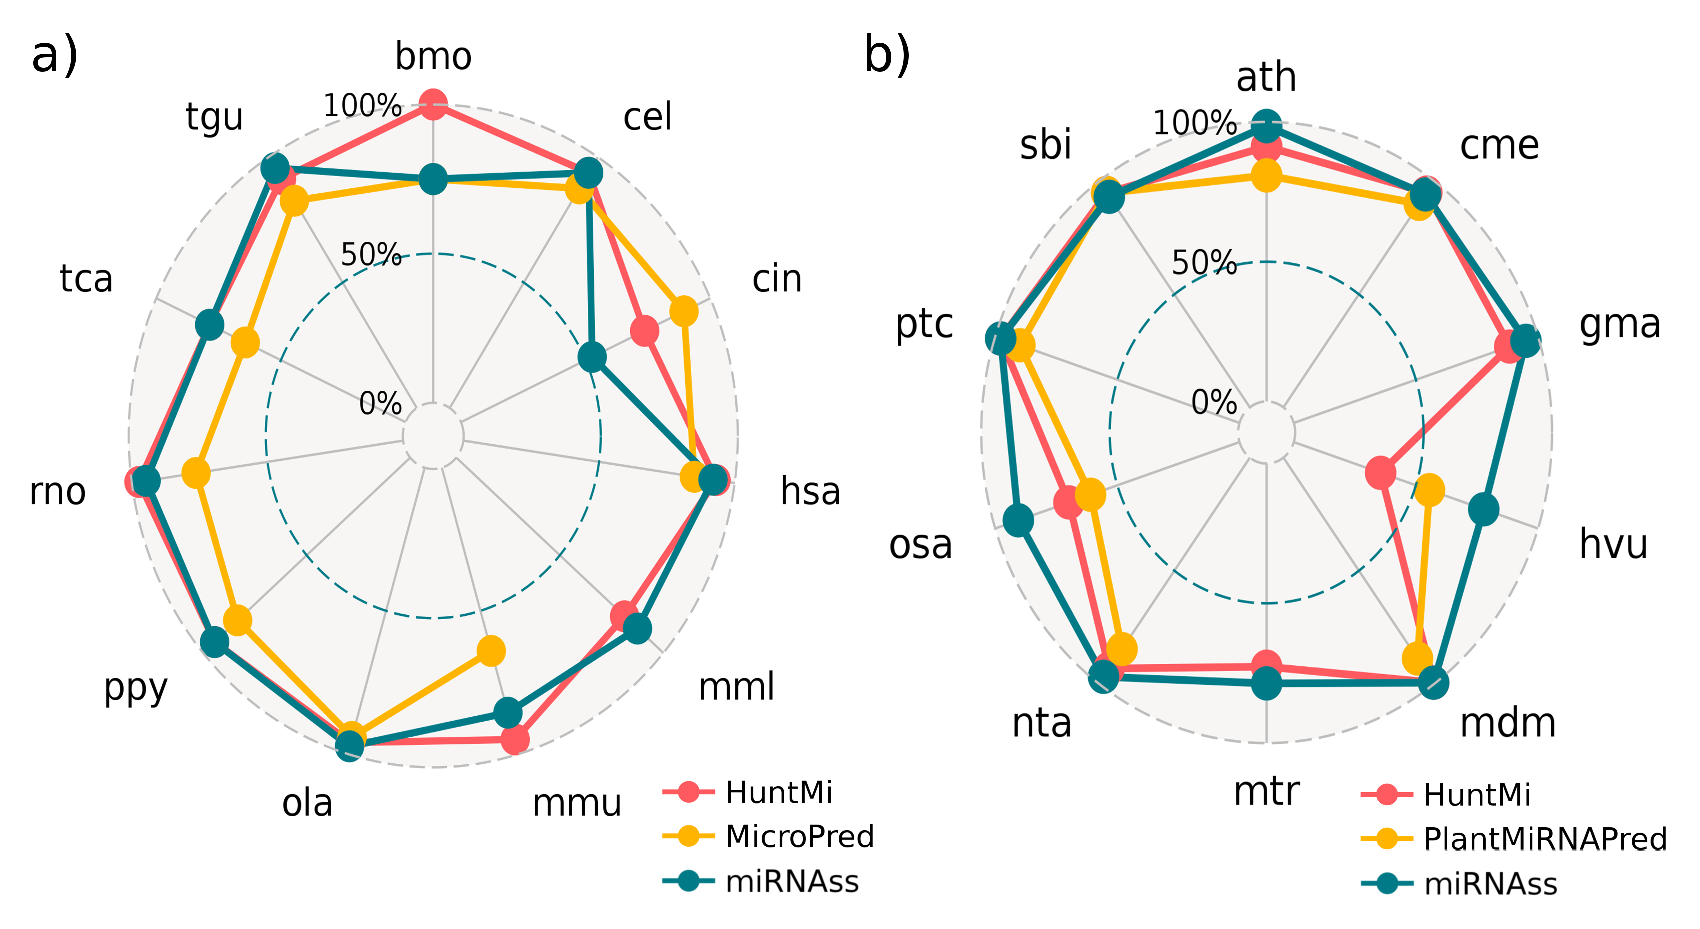
\includegraphics[width=0.6\linewidth]{delta_mirbase_radar.eps}
	\caption{Sensitivity obtained with several state-of-the-art classifiers in: a) animal species, and b) plant species. The distance of each point to the center measures the sensitivity obtained on each species.}
	\label{fig:deltaRadar}
\end{figure}
%*****************************************************************************************

The $S^{+}$ obtained on each species is shown in Fig.~\ref{fig:deltaRadar}, where each classifier is mapped with a different color across a radar plot. In the animals dataset, miRNAss outperformed microPred in almost all the species. In the human dataset, miRNAss obtained higher $S^{+}$ than microPred, which, as mentioned above, was specifically designed for humans. Compared with HuntMi, miRNAss obtained higher $S^{+}$ in 4 species, HuntMi produced better results in 4 species, and the results obtained were the same in 3 species. In plants, miRNAss outperformed PlantMiRNAPred in almost all the species. Compared with HuntMi, miRNAss had a better $S^{+}$ in 8 species, while HuntMi slightly outperformed miRNAss in only 2 species (\textit{Cucumis melo} and \textit{Sorghum bicolor}).
To analyze if there were significant differences between classifiers, Nemenyi tests \citep{nemenyi1962distribution} were conducted for animals and plants datasets ($p<0.05$). In animals species, HuntMi and miRNAss produced equivalent results, but both performed better than microPred. In plant species, miRNAss obtained the lowest rank (the best) and a significant difference with PlantMiRNAPred; however, the difference with HuntMi was not statistically significant.

Supervised methods make extensive use of labeled data, not only for training but also for finding the optimal hyper-parameters and thresholds. On the contrary, miRNAss was built over the hypothesis that labeled examples are scarce, unreliable, and not representative of the whole class, which is actually a more realistic scenario for this prediction task. Therefore, it should be noted that, even under these disadvantageous conditions, miRNAss obtained significantly better results than MicroPred and PlantMiRNAPred, and equivalent results to those produced by HuntMi, being, however, many times faster.

\subsection{Few labeled examples}
In order to depict a more realistic scenario, in which the number of known examples is very low, the five datasets used in the last tests were sampled in a train-test validation scheme with a varying percentage of labeled sequences. The percentage of labeled examples was reduced from 20\% to 2\%, with a step of 2\%. The labeled examples were randomly selected and the tests were repeated 200 times for each percentage to estimate confidence intervals. In the Fig.~\ref{fig:fewSamples:huntmi}, curves of expected $F_{1}$ with confidence intervals of 0.05 were estimated for comparison. In the human dataset, the $F_{1}$ is almost 10\% higher for miRNAss, regardless of the percentage of labeled sequences. In the Arabidopsis dataset, where the number of positive examples sequences was lower, the differences in favor of miRNAss were the highest at the lower percentages of labeled examples, which indicates that miRNAss can effectively identify the positive class even  with a very low number of labeled examples. The same trends are observed in the animals, plants, and virus datasets (see Supplementary Figure~S6).
These results not only show that miRNAss is capable of outperforming supervised methods when the number of labeled examples is low, but also that the error rates estimated using a high proportion of labeled examples are very different from those obtained in more realistic scenarios.

A further step towards a more realistic prediction task consists in using only positive examples. Under these conditions, miRNAss was compared with miRank \citep{xu2008microrna}, which was designed to work with an extremely small number of positive examples. Datasets provided by the original author were used: 533 human pre-miRNAs and 1000 non-miRNA sequences. To make a fair comparison, both method used the feature set of miRank. This set is composed by 32 triplets \citep{xue2005classification}, normalized MFE, normalized base pairing propensities of both arms and normalized loop length. A varying number of positive examples (1, 2, 4, 8, 16, 32, 64, and 128) were labeled and the rest of the sequences were left unlabeled in order to measure the error rates. As the results depend on a random sampling of the sequences, this procedure was repeated 1000 times for each number of labeled examples. MiRank provides as output a continuous score; therefore, the prediction scores obtained with miRNAss were not thresholded. The area under the precision-recall curve was calculated (AUCPR), since it takes all possible thresholds into account \citep{bradley1997use}.
%****************************************************************************************
\begin{figure}[tpb]
	\centering
	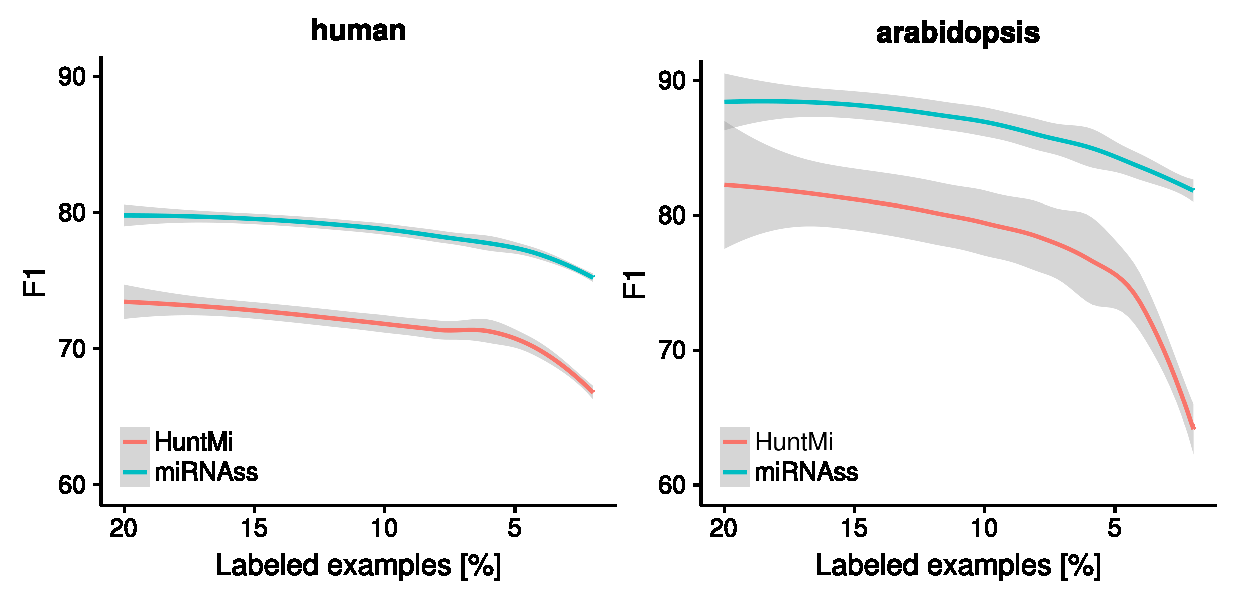
\includegraphics[width=0.6\linewidth]{few_samples_huntmi.eps}
	\caption{Curves of $F_{1}$ obtained by decreasing the percentage of labeled sequences. Shaded regions represent confidence intervals of the estimation with local regression (LOESS) at $p < 0.05$.}
	\label{fig:fewSamples:huntmi}
\end{figure}
%****************************************************************************************

In this test, the 5\% of the estimated $n_{-}$ is automatically labeled by miRNAss as negative examples to initiate the algorithm. As it is shown in the Figure~S1 of Supplementary Material, miRNAss is not sensitive to this parameter. Figure~\ref{fig:miRank} presents a box plot with the distribution of AUCPR obtained by each classifier with a different number of labeled examples. MiRNAss maintained an almost constant AUCPR, irrespective of the number of labeled pre-miRNAs, while the performance of miRank decreased markedly. In addition, the values of AUCPR for miRNAss showed a little dispersion compared with miRank, which becomes very unstable when the number of labeled examples decreases. This instability may be produced by positive examples that are close to the frontier of the class, causing miRank to fail to set the decision boundary. The semi-supervised miRNAss algorithm correctly found the low-density regions that separate miRNAs from the rest of the sequences, regardless of the examples provided.

\subsection{Real prediction in whole genomes} \label{sec:results:genome-wide}
MiRNAss was tested with the genome-wide data of three well-known genomes: \textit{Arabidopsis thaliana}, \textit{Caenorhabditis elegans} and \textit{Anopheles gambiae}, to reproduce all the conditions of a real prediction task. Previous works tested methods on genome-wide data from single species \citep{lai2003computational, bentwich2005identification, adai2005computational, huang2007mirfinder, billoud2014computational}, but in this study we have processed three complete genomes and made all genome-wide datasets available for testing machine learning methods in pre-miRNAs prediction.
The whole genomes were processed to extract all the existing stem-loops. For this purpose, all the chromosomes and mitochondrial genes were split in 600-nt-long windows, with a 100-nt overlap. The secondary structure of these sequences was predicted with RNAfold \citep{lorenz2011viennarna}. Then, all stem loops of at least 60 nt in length and 16 matched base pairs found in these structures were pruned and saved, taking care of deleting duplicated cases.
This process left a total of 1,356,616 stem-loops of \textit{A. thaliana}; 1,698,859 stem-loops of \textit{C. elegans}; and 4,276,188 stem-loops of \textit{A. gambiae}. BLAST \citep{camacho2009blast+} was used to match all the well-known pre-miRNAs annotated in mirBase v21 with the extracted stem-loops. This defined a total of 304, 249 and 66 hairpins as positive set for \textit{A. thaliana}, \textit{C. elegans}, \textit{A. gambiae}, respectively.
Two sets of features were extracted from the three genomes. The first one (FS1) is the same used in Section~\ref{sec:results}.1, to make a fair comparison with one of the methods. The second feature set (FS2) is an extended set composed by almost all features proposed for pre-miRNA prediction in literature. FS2 was calculated with miRNAfe \citep{yones2015mirnafe} and each feature vector resulted in 79 elements. For more details on the feature sets see Supplementary Material, Section~S4. A 10-fold cross-validation (CV) scheme was used to measure miRNAss performance with averaged ROC curves.
%****************************************************************************************
\begin{figure}[tpb]
	\centering
	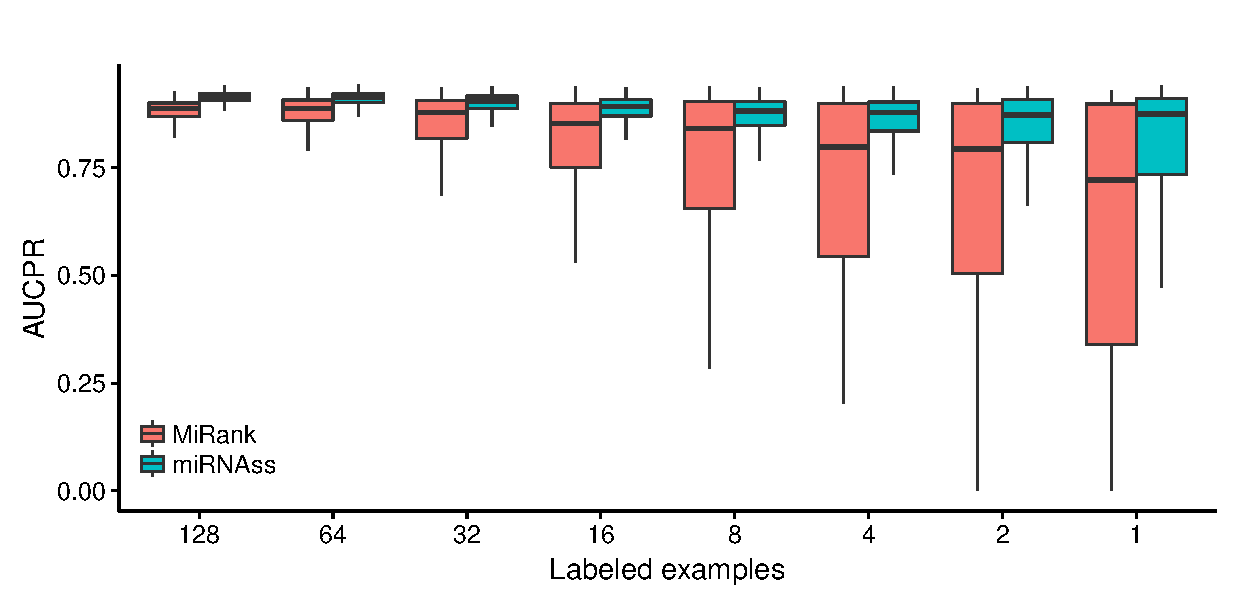
\includegraphics[width=0.6\linewidth]{few_samples_miRank.eps}
	\caption{Box plot of the areas under the curve obtained by miRNAss and miRank, with a different number of positive training samples.}
	\label{fig:miRank}
\end{figure}
%****************************************************************************************

Many pre-miRNA prediction algorithms were tested on these datasets to compare their performance with miRNAss. We have tried eleven predictors, but most of them failed with genome-wide data or their servers are not working. The only five predictors that could be used for these comparisons were HuntMi, Mirident \citep{liu2012integrated}, HHMMiR \citep{kadri2009hhmmir}, MiRPara \citep{wu2011mirpara} and miR-BAG \citep{jha2012mir}. The first two methods produce hard class assignments (not scores), and that is why they are points in ROC figures. Instead, since MiRPara, miR-BAG, HHMMiR and miRNAss provide a score for each sequence, complete ROC curves can be drawn. MiR-BAG was not run on \textit{A. thaliana} because it does not provide a model for plants. The output scores obtained with this method can only take four possible values, therefore, the ROC curves have straight lines. These results can be seen in Figure~\ref{fig:ROC}.
In the \textit{A. thaliana} genome, it can be seen that the miRNAss ROC curves are above miRPara and HHMMiR curves for all threshold values. It should be noted that Mirident, in spite of having the highest true positive rate (sensitivity), it also has the highest false positive rate. HuntMi is more balanced, having a high true positive recognition and a moderate number of false positives. Anyway, it is below miRNAss with both feature sets.
In the \textit{C. elegans} genome, a similar analysis can be done for HuntMi and Mirident. In this dataset, miR-BAG generates a ROC curve similar to the curve of MiRPara, both below the rest of the curves. HHMMiR presents a better performance than these methods, but again it is outperformed by miRNAss.
In the case of the \textit{A. gambiae} genome, performance of miRNAss with FS1 is more distant to the FS2. MiR-BAG and HHMMiR generate a curve similar to the obtained by miRNAss with FS2, far below the one obtained with FS1. The ROC curve with FS1 shows that, in the upper left corner, miRNAss can provide the best balance between sensitivity and false positive rate. In fact, this is nearly an ideal ROC curve.
%****************************************************************************************
\begin{figure*}[tpb]
	\centering
	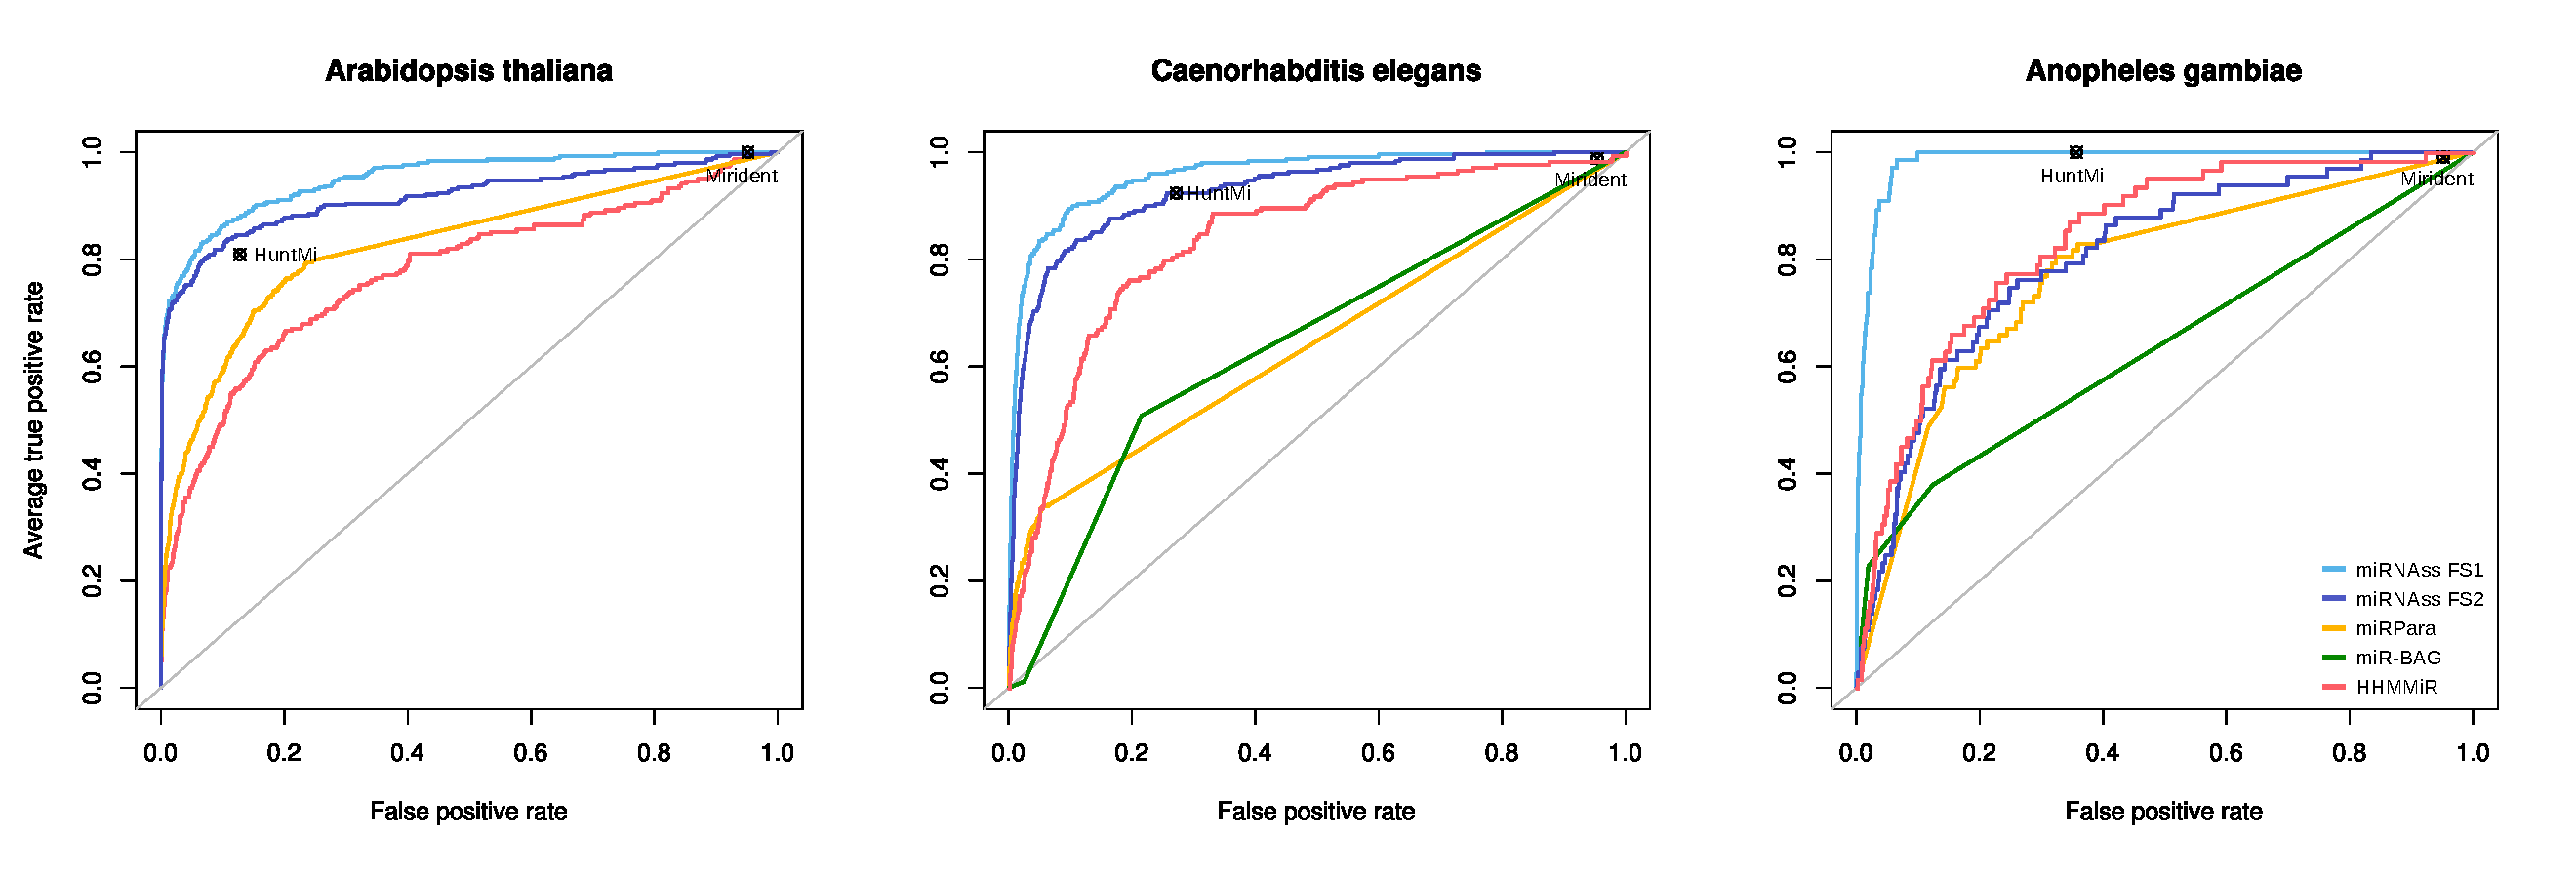
\includegraphics[width=\linewidth]{genome-wide_ROC.eps}
	\caption{ROC curves for comparisons with state-of-the-art methods on genome-wide data from three species. The points show the performance achieved by methods that only return hard class assignments.}
	\label{fig:ROC}
\end{figure*}
%****************************************************************************************

Finally, as a summary of the comparative analysis, Table~\ref{tab:wholegenome} presents more results of practical interest. The same methods and species of Figure~\ref{fig:ROC} are here analyzed according to global performance and the total number of candidates that each method returns using their default threshold values, that is, the sum of true positives and false positives ($TPFP$). It can be seen that miRNAss outperforms all the methods in the three genomes. Mirident is the method with the lowest performance, for all species. This is because it labels as positive almost all examples, which is reflected in a very high sensitivity, but without practical utility given the number of candidates provided. MiR-BAG has a better but still poor performance in both species. HHMMiR and miRPara predict very few candidates, with high specificity at the cost of a very low sensitivity. HuntMi, instead, allows obtaining more balanced results, with the second best performance. However, for example in \textit{A. gambiae}, it returns a number of false positives more than 5 times higher than those returned by miRNAss.

These results allow us to state that miRNAss outperforms supervised methods in a realistic classification setup.
Artificially defined negative examples are used to train supervised models and, since these examples are not representative of the vast diversity of the negative class, the models fail to discard non-miRNA sequences correctly. By contrast, miRNAss can better take advantage of the very large number of unlabeled sequences to more tightly fit the decision boundary around the pre-miRNAs, discarding the rest of the sequences.
%*******************************************************************************************
\begin{table}[tpb]
	\centering
	\caption{Geometric mean of sensitivity and specificity ($\bar{G}$) and true$+$false positives ($TPFP$) on the three whole genome test. \label{tab:wholegenome}}
	\begin{tabular}{@{}lrcrcrc@{}} \toprule
		&	\multicolumn{2}{c}{\textit{A. thaliana}}
		&	\multicolumn{2}{c}{\textit{C. elegans}}
		&	\multicolumn{2}{c}{\textit{A. gambiae}} \\
		\multirow{2}{*}{Classifier}	&	 $TPFP$		&	 $\bar{G}$
						&	 $TPFP$			&	 $\bar{G}$
						&	 $TPFP$			&	 $\bar{G}$	\\\midrule
		{\small Mirident}	&	 1,294,648		&	 22.05 \%
					&	 1,617,221		&	 21.29 \%
					&	 4,068,431		&	 21.86 \%	\\
		{\small miR-BAG}	&	 -			&	 -
					&	 375,011		&	 63.14 \%
					&	 495,231		&	 57.62 \%	\\
		{\small miRPara}	&	 2,755			&	 47.95 \%
					&	 11,712			&	 53.79 \%
					&	 283,232		&	 72.48 \%	\\
		{\small HHMMiR}		&	 45,104			&	 69.07 \%
					&	 40,318			&	 73.29 \%
					&	 91,093			&	 74.07 \%	\\
		{\small HuntMi}		&	 173,906		&	 84.00 \%
					&	 462,203		&	 82.00 \%
					&	 1,456,590		&	 80.20 \%	\\
		{\small MiRNAss}	&	 134,369		&	 \textbf{84.82 \%}
					&	 164,557		&	 \textbf{87.61 \%}
					&	 258,096		&	 \textbf{93.34 \%}	\\\bottomrule
	\end{tabular}
\end{table}
%*********************************************************************************************

\section{Conclusions} \label{sec:conclusions}
In this study, we presented a new pre-miRNA prediction method called miRNAss, which uses a semi-supervised approach to face the problem of scarce and unreliable training samples. The experiments conducted in a forced supervised setup showed that miRNAss can achieve the classification rates of the best state-of-the-art methods in standard cross-validation tests, in shorter times. The proposed method was also tested under conditions that are closer to a real prediction task, where the number of labeled sequences is decreased. In these tests, miRNAss clearly outperformed the best available state-of-the-art supervised method, producing better results than a method that was specially designed to work under these conditions. The automatic search for negative examples proved to work well.
The final test over all the stem-loops of three genomes using two different sets of features raises many important considerations. First of all, miRNAss widely outperforms the classification rates of supervised approaches. In addition, miRNAss proved to be efficient and scalable for handling over four million sequences. The results on this test also proved an important hypothesis made at the beginning of this study: the negative examples that are used to train many state-of-the-art prediction methods are not representative of the whole non-miRNA class. While those methods achieved very high error rates in cross-validation tests with an artificially defined negative class, the performance falls when they have to face the wide range of sequences that can be found in any genome. By contrast, miRNAss automatically searches for a wide variety of negative examples to initiate the algorithm. Then, miRNAss strives to take advantage of the distribution of unlabeled samples. As a result, it is capable of fitting tight decision boundaries around the pre-miRNAs using only a few positive examples.

\section*{Funding}
This work was supported by Consejo Nacional de Investigaciones Cient\'ificas y T\'ecnicas [PIP 2013 117], Universidad Nacional del Litoral [CAI+D 2011 548, 2016 082] and Agencia Nacional de Promoci\'on Cient\'ifica y Tecnol\'ogica [PICT 2014 2627], Argentina.


\bibliographystyle{natbib}
\bibliography{mirnass}
\end{document}
